\documentclass[11pt,oneside,french]{book}
\usepackage[margin=1.2in]{geometry}
\usepackage[toc,page]{appendix}
\usepackage{graphicx}
% \usepackage{natbib}
\usepackage{float}
\usepackage{lipsum}
\usepackage{changepage}
\usepackage{hyperref}
\usepackage{textcomp}
\usepackage{hyperref}
\usepackage[utf8]{inputenc}
\usepackage[T1]{fontenc}
\usepackage[english]{babel}
\usepackage{caption}
\usepackage{background}
\usepackage{amsmath}
\usepackage{pdfpages}
\usepackage{biblatex}
\usepackage{titletoc}  % Add titletoc package
\addbibresource{sample.bib}

\usepackage{glossaries}
\newacronym{DLIA}{DLIA}{DeepVolt Location Intelligence Assistant}
% Add a page for acronyms
\printglossary[type=\acronymtype, title={List of Acronyms}]

\begin{document}

\captionsetup[figure]{margin=1.5cm,font=small,labelfont={bf},name={Figure},labelsep=colon,textfont={it}}
\captionsetup[table]{margin=1.5cm,font=small,labelfont={bf},name={Tableau},labelsep=colon,textfont={it}}
\SetLipsumDefault{1}

\frontmatter

\begin{titlepage}
\backgroundsetup{
scale=1,
angle=0,
opacity=1,
contents={
\includegraphics[width=\paperwidth,height=\paperheight]{figures/page_garde.jpg}}
}

\begin{center}
\end{center}

\end{titlepage}

\newpage
\backgroundsetup{contents={}}

\begin{center}
\end{center}

\newpage
\chapter*{\Large \center Dédicaces}

Je dédie ce travail :

\vspace{1em}

\noindent
À mes parents, pour leur amour inconditionnel, leurs sacrifices silencieux et leur soutien constant tout au long de mon parcours académique. Leur confiance m’a donné la force d’aller jusqu’au bout.

\vspace{1em}

\noindent
À ma famille, pour leur présence, leurs encouragements et leur patience, même dans les moments les plus exigeants de ce projet.

\vspace{1em}

\noindent
À mes amis et collègues, pour leur aide, leurs conseils, et les bons moments partagés qui ont rendu cette expérience plus agréable et motivante.

\vspace{2em}


\hfill\textbf {Aziz Aydi}\\

\chapter*{\Large \center remerciement}

Avant toute chose, je tiens à exprimer ma profonde gratitude à tous ceux qui ont contribué de près ou de loin à la réussite de ce projet de fin d'études.

Je remercie sincèrement \textbf{Madame Houda Jouini Chaabouni}, mon encadrante académique, pour sa disponibilité, ses conseils méthodologiques et son encadrement rigoureux tout au long de cette expérience. Son expertise et ses remarques constructives ont grandement enrichi ce travail.

Je tiens également à remercier \textbf{Monsieur Hichem Aidi}, pour sa confiance, son accompagnement technique et son suivi professionnel qui m'ont permis de m’intégrer dans une logique projet concrète et enrichissante.

Je n’oublie pas l’ensemble du corps professoral de l’école d’ingénieurs \textbf{ESPRIT}, pour la qualité des enseignements dispensés, qui m’ont permis d’acquérir les compétences nécessaires à la réalisation de ce projet.

Enfin, je remercie chaleureusement tous mes collègues, camarades, amis et proches pour leur soutien moral, leur entraide et leurs encouragements constants.

\bigskip

\hfill \textit{À toutes et à tous, merci.}

\hfill\textbf {Aziz Aydi}\\
\chapter*{\Large \center Resumé}
Dans le cadre de ce projet de fin d’études, nous avons conçu, développé et déployé une plateforme web baptisée \textbf{Swift Helpers}, destinée à mettre en relation des clients avec des prestataires de services (helpers) dans un environnement numérique fluide, intuitif et sécurisé.

Le projet a été mené selon une démarche agile, découpée en plusieurs sprints successifs. Chaque sprint a couvert une fonctionnalité majeure du système : gestion des comptes clients, gestion des prestataires, traitement des ordres de mission, supervision administrative, et enfin déploiement de l’ensemble du système dans un environnement conteneurisé à l’aide de Docker.

Sur le plan technique, la solution repose sur un backend développé avec \textbf{Django REST Framework}, un frontend en \textbf{Angular}, une base de données \textbf{PostgreSQL}, et un déploiement orchestré par \textbf{Docker} et \textbf{NGINX}. Ce socle technologique garantit modularité, performance et maintenabilité.

Ce rapport retrace toutes les étapes de réalisation du projet, de l’analyse initiale des besoins jusqu’à la mise en production, tout en mettant en évidence les choix techniques, les modèles de données, les diagrammes UML et les interfaces utilisateur développées.

\noindent Mots-clés: Développement web, Swift Helpers, plateforme de services, Django, Angular, PostgreSQL, API REST, Docker, architecture logicielle, méthode agile, déploiement.\\[1mm]
\rule[1em]{38em}{0.5pt}

\tableofcontents
\listoffigures

% List of Abbreviations
\newpage
\begin{center}
  \textbf{\Large List of Abbreviations}
\end{center}

\begin{description}
  \item[AC] Alternating Current
  \item[AD] Direct Current
  \item[ADDT] Annual Average Daily Traffic
  \item[AI] Artificial Intelligence
  \item[API] Application Programming Interface
  \item[AWS] Amazon Web Services
  \item[CPO] Charge Point Operator
  \item[DLIA] DeepVolt Location Intelligence Assistant
  \item[E-Mobility] Electromobility
  \item[EV] Electric Vehicle
  \item[EVCS] Electric Vehicle Charging Station
  \item[IDE] Integrated Development Environment
  \item[MLOps] Machine Learning Operations
  \item[ML] Machine Learning
  \item[MVP] Minimum Viable Product
  \item[OLS] Ordinary Least Squares
  \item[POI] Point of Interest
  \item[SaaS] Software as a Service
  \item[TIF] Tagged Image Format
\end{description}

\mainmatter

\addcontentsline{toc}{chapter}{Introduction}
\chapter*{\Large \center Introduction générale}

Dans un monde en constante évolution numérique, les plateformes de services à la demande se multiplient pour répondre aux besoins croissants d’efficacité, de flexibilité et de réactivité. Qu’il s’agisse de mise en relation entre particuliers ou de solutions destinées à des structures professionnelles, ces systèmes doivent être pensés pour offrir à la fois une expérience utilisateur fluide, une architecture technique robuste et une évolutivité assurée.

C’est dans ce contexte qu’intervient le projet \textbf{Swift Helpers}, développé dans le cadre de mon projet de fin d’études au sein de la spécialité Génie Logiciel de l’école d’ingénieurs ESPRIT. Ce projet vise à concevoir, développer et déployer une application web complète permettant la gestion d’un réseau de prestataires de services, avec une attention particulière portée à la simplicité d’utilisation, à la modularité technique et à l’automatisation des processus métier.

Le développement de la plateforme s’inscrit dans une démarche agile, structurée en sprints, couvrant toutes les étapes de réalisation : de l’analyse des besoins à l’implémentation des fonctionnalités, jusqu’au déploiement sur un environnement de production Dockerisé. Le système repose sur un backend \textbf{Django REST}, un frontend \textbf{Angular}, une base de données \textbf{PostgreSQL}, et une infrastructure conteneurisée à l’aide de \textbf{Docker}.

Ce projet m’a offert l’opportunité d’appliquer concrètement les compétences acquises tout au long de ma formation, que ce soit en architecture logicielle, en développement fullstack, en conception orientée objet ou en gestion de projet. Il représente également une première immersion dans les exigences réelles d’un système exploitable par des utilisateurs finaux.

Ce rapport présente, dans un premier temps, le contexte général du projet et son périmètre fonctionnel. Il détaille ensuite les différentes phases de développement, organisées par sprint, avant de conclure par le processus de déploiement, les choix techniques effectués, et les perspectives d’évolution du système.

\chapter{Contexte générale du projet }
% Guidance on how to write an abstract/summary provided by Nature: https://cbs.umn.edu/sites/cbs.umn.edu/files/public/downloads/Annotated_Nature_abstract.pdf

\section*{Introduction}

Dans ce premier chapitre, nous présentons une vue d’ensemble de notre projet de fin d’études. Nous décrivons tout d’abord l’environnement du stage, notamment l’organisme d’accueil et son domaine d’activité. Ensuite, nous établissons le contexte du projet en mettant en lumière les besoins identifiés, les objectifs visés ainsi que les enjeux métier associés. Cette introduction couvre également une étude de l’existant et des travaux similaires ou connexes ayant inspiré ou orienté notre démarche. Enfin, nous concluons le chapitre par un résumé des contributions prévues dans le cadre de ce projet, tant sur le plan technique que fonctionnel. \\

\section {Contexte académique }

Ce projet de fin d’études s’inscrit dans le cadre de ma formation en cinquième année, spécialité Génie Logiciel, au sein de l’École Supérieure Privée d'Ingénierie et de Technologie (ESPRIT). Il représente l’aboutissement de cinq années d’apprentissage intensif, alliant théorie et pratique.\\

\noindent Ce projet marque la clôture officielle de mon parcours académique et constitue une transition déterminante vers le monde professionnel. À travers ce travail, j’ai eu l’opportunité d’appliquer de manière concrète mes compétences techniques et méthodologiques au sein d’un environnement réel, tout en répondant à des besoins métier précis. Il s’agit d’une étape essentielle dans la formation de l’ingénieur, car elle permet de démontrer sa capacité à concevoir et développer une solution logicielle complète, robuste et évolutive, conforme aux standards du domaine.\\

\section{Organisme d’accueil}

inotekplus...


\section{Contexte Du Projet} 
Dans un monde de plus en plus tourné vers la digitalisation des services, les plateformes de mise en relation entre clients et prestataires connaissent une forte croissance. Le besoin de solutions intelligentes, automatisées et flexibles devient essentiel pour répondre aux exigences d’efficacité, de rapidité et de traçabilité des prestations. C’est dans ce contexte que s’inscrit ce projet de fin d’études, qui consiste à développer une plateforme de réservation de services intégrant un chatbot conversationnel, une gestion complète des ordres de mission, ainsi qu’un système automatisé de suivi et de facturation.


\\
\section{Étude de l’existant}

Dans le domaine des services à la demande, plusieurs plateformes numériques telles que \textbf{TaskRabbit}, \textbf{Thumbtack}, \textbf{HomeAdvisor} ou encore \textbf{Jiffy} (plus active au Canada) permettent aux clients de réserver des services ponctuels auprès de prestataires indépendants. Ces solutions sont bien implantées sur le marché nord-américain et ont réussi à capter une part significative des utilisateurs en quête de services rapides et flexibles.

\subsection*{Points forts des solutions existantes}
\begin{itemize}
  \item \textbf{Interface conviviale et intuitive} : la majorité de ces plateformes proposent des applications mobiles et des interfaces web modernes, facilitant la recherche, la réservation et le suivi des services.
  \item \textbf{Large éventail de services} : qu’il s’agisse de ménage, jardinage, plomberie, petits travaux ou livraison, ces solutions couvrent une grande diversité de besoins.
  \item \textbf{Notation des prestataires} : les systèmes d’évaluation et d’avis clients permettent de renforcer la confiance entre utilisateurs.
  \item \textbf{Messagerie intégrée} : certaines plateformes proposent une messagerie sécurisée pour échanger avant l’intervention.
  \item \textbf{Paiement en ligne sécurisé} : la majorité offre une intégration fluide des paiements électroniques, ce qui améliore la rapidité et la sécurité des transactions.
\end{itemize}

\subsection*{Limites et faiblesses constatées}

Malgré leurs atouts, ces solutions présentent des limites importantes, notamment dans le contexte canadien et plus spécifiquement en \textbf{Alberta}, où les besoins des PME, franchises locales ou coopératives de services sont plus spécifiques :

\begin{itemize}
  \item \textbf{Absence de chatbot conversationnel} : l’interaction client est souvent limitée à des formulaires statiques qui manquent de souplesse. Aucune solution étudiée ne propose un chatbot intelligent capable de comprendre le besoin, poser des questions de clarification et générer automatiquement un ordre.
  
  \item \textbf{Suivi opérationnel basique} : une fois le service réservé, le suivi de l’intervention (départ, arrivée, exécution, fin) est souvent flou. Il manque une traçabilité structurée permettant aux prestataires et aux clients de suivre chaque étape du cycle de mission.

  \item \textbf{Facturation manuelle ou partielle} : peu de solutions offrent une facturation automatique déclenchée par l’état d’avancement réel du travail. Cela implique souvent une charge administrative pour le prestataire et des délais pour le client.

  \item \textbf{Manque de support pour le modèle multi-entité (multi-tenancy)} : dans un contexte B2B comme en Alberta, où des entreprises peuvent gérer plusieurs sites ou entités (par exemple, un réseau de franchisés ou de coopératives), il est crucial que chaque entité ait un espace de gestion indépendant. Or, la majorité des plateformes sont pensées pour un modèle centralisé, ce qui limite leur capacité d’adaptation à ce type de structure.

  \item \textbf{Peu d’adaptation aux spécificités locales} : au Canada, et particulièrement en Alberta, des aspects comme la gestion des taxes (TPS/TVH), les devises multiples, les conditions climatiques (ex. : services saisonniers) ou encore les normes professionnelles provinciales sont souvent négligés par les solutions génériques importées des États-Unis.
\end{itemize}

\medskip

Ainsi, bien que le marché canadien — notamment albertain — bénéficie déjà de plusieurs plateformes de services à la demande, \textbf{il subsiste un besoin réel pour une solution plus intelligente, automatisée, adaptable aux réalités professionnelles locales et capable de gérer plusieurs entités en toute autonomie}.

\section{Problématique}

L’analyse des solutions existantes a permis de mettre en évidence plusieurs lacunes majeures, en particulier dans le contexte professionnel et géographique ciblé par ce projet : la province de l’Alberta au Canada. Bien que certaines plateformes offrent des fonctionnalités de base intéressantes, elles ne répondent pas totalement aux besoins spécifiques des entreprises locales ou des structures multi-sites souhaitant optimiser leur gestion de services sur le terrain.

\medskip

Ainsi, plusieurs problématiques clés émergent :

\begin{itemize}
  \item \textbf{Comment améliorer la collecte des besoins client de manière fluide et interactive ?}  
  Les formulaires statiques montrent leurs limites. Il devient nécessaire d’intégrer un agent conversationnel (chatbot) intelligent capable de dialoguer avec le client pour cerner précisément ses attentes et générer automatiquement une demande structurée.

  \item \textbf{Comment permettre une gestion personnalisée et indépendante des données pour chaque entité cliente ?}  
  Dans un modèle multi-entité (multi-tenancy), chaque entreprise, franchise ou partenaire doit pouvoir gérer ses clients, ses prestataires et ses ordres de manière autonome, sans interférence avec les autres entités hébergées sur la même plateforme.

  \item \textbf{Comment structurer le suivi opérationnel d’un ordre de mission ?}  
  Il est essentiel d’introduire une traçabilité complète du service : indication du départ du prestataire, début de l’intervention, fin de la mission, et génération automatique d’une preuve d’exécution.

  \item \textbf{Comment automatiser la facturation en lien direct avec l’état d’avancement de la prestation ?}  
  Une facturation manuelle est source d’erreurs, de retards et de surcharge administrative. Un mécanisme automatisé lié à la clôture de la mission permettrait d’optimiser ce processus.
\end{itemize}

\medskip

Ces problématiques illustrent le besoin d’une solution plus intelligente, modulaire et adaptée aux spécificités du marché canadien, en particulier pour les structures de services réparties sur plusieurs territoires ou clients B2B.
demographic data.\\[1mm]

\section{Choix de la méthodologie de développement}

\subsection{Étude comparative des méthodologies de développement}

Dans l’évaluation des différentes méthodologies de développement pour notre application, nous avons mené une étude comparative approfondie afin d’évaluer leur pertinence et leur alignement avec les objectifs du projet. Voici une analyse de plusieurs méthodologies reconnues :

\subsubsection*{Méthodologie Waterfall}
\textbf{Caractéristiques} :\\
La méthodologie Waterfall suit une approche linéaire et séquentielle avec des phases distinctes telles que la collecte des exigences, la conception, l'implémentation, les tests et la maintenance.

\textbf{Avantages} :
\begin{itemize}
    \item Processus bien défini et structuré.
    \item Jalons et livrables du projet clairement établis.
    \item Convient aux projets avec des exigences stables et bien comprises.
\end{itemize}

\textbf{Inconvénients} :
\begin{itemize}
    \item Flexibilité limitée pour intégrer des changements.
    \item Implication minimale des parties prenantes avant les étapes finales.
    \item Risque élevé de révisions coûteuses si les exigences changent en fin de projet.
\end{itemize}

\subsubsection*{Méthodologie Agile}
\textbf{Caractéristiques} :\\
Les méthodologies Agile, telles que \textit{Scrum} et \textit{Kanban}, mettent l'accent sur un développement itératif et incrémental, une collaboration étroite avec les parties prenantes et une capacité d'adaptation aux changements.

\textbf{Avantages} :
\begin{itemize}
    \item Flexibilité pour intégrer des exigences évolutives.
    \item Feedback et engagement réguliers des parties prenantes.
    \item Temps de mise sur le marché plus rapide et capacité à délivrer de la valeur plus tôt.
\end{itemize}

\textbf{Inconvénients} :
\begin{itemize}
    \item Nécessite une forte implication des parties prenantes tout au long du projet.
    \item Peut manquer de documentation suffisante pour la conformité réglementaire.
    \item Courbe d'apprentissage initiale pour les équipes passant des méthodologies traditionnelles.
\end{itemize}

\subsubsection*{Méthodologie Lean Startup}
\textbf{Caractéristiques} :\\
La méthodologie Lean Startup se concentre sur la validation rapide des hypothèses grâce à des expérimentations itératives et aux retours des clients, afin de concevoir des produits ou services répondant aux besoins réels des utilisateurs.

\textbf{Avantages} :
\begin{itemize}
    \item Itérations rapides et validation des idées.
    \item Réduction des ressources gaspillées sur des fonctionnalités à faible valeur ajoutée.
    \item Accent mis sur l'apprentissage et l’ajustement en fonction des retours du marché.
\end{itemize}

\textbf{Inconvénients} :
\begin{itemize}
    \item Risque de mise à l’échelle prématurée sans validation suffisante.
    \item Dépendance à une culture d'expérimentation et de prise de risques.
    \item Difficultés potentielles dans la mesure des progrès et des indicateurs de succès.
\end{itemize}

\subsubsection*{Méthodologie Spiral}
\textbf{Caractéristiques} :\\
La méthodologie Spiral combine des éléments de développement itératif et de gestion des risques, permettant un développement incrémental tout en abordant les risques liés au projet.

\textbf{Avantages} :
\begin{itemize}
    \item Intégration de la gestion des risques dans le processus de développement.
    \item Flexibilité pour revisiter et affiner les exigences du projet de manière itérative.
    \item Convient aux projets avec une forte incertitude ou des exigences évolutives.
\end{itemize}

\textbf{Inconvénients} :
\begin{itemize}
    \item Complexité accrue en raison de la nature itérative du processus.
    \item Risque d'élargissement du périmètre si les risques ne sont pas gérés efficacement.
    \item Nécessite une expertise solide en gestion de projet et en analyse des risques.
\end{itemize}

\subsection{Méthodologie adoptée}

Pour le développement de notre application web, la \textbf{méthodologie Agile Scrum} a été choisie comme méthode privilégiée. Agile Scrum offre une approche collaborative et itérative particulièrement adaptée aux projets de développement logiciel, notamment ceux avec des exigences évolutives et un besoin de flexibilité.

Cette méthodologie permet de favoriser la collaboration entre les parties prenantes et les membres de l'équipe, tout en garantissant une capacité d'adaptation rapide aux changements et une livraison incrémentale de valeur tout au long du projet.
\section*{Technologies utilisées}

Le projet \textit{Swift Helpers} s’appuie sur un ensemble de technologies modernes soigneusement sélectionnées pour leur stabilité, leur adoption dans l’industrie, et leur capacité à répondre aux exigences du projet.

\subsection*{Django (Backend)}
\begin{figure}[H]
\centering

\includegraphics[width=2.5cm]{figures/django.png}
\end{figure}
\noindent
\textbf{Django} a été choisi pour la construction du backend grâce à sa rapidité de développement, sa sécurité intégrée et son ORM efficace. Il facilite la création d’API REST en association avec \texttt{Django REST Framework} et permet une structuration claire du code serveur.

\subsection*{Angular (Frontend)}
\begin{figure}[H]
\centering

\includegraphics[width=2.5cm]{figures/angular.png}
\end{figure}
\noindent
\textbf{Angular} est un framework robuste basé sur TypeScript, idéal pour développer des applications web dynamiques et modulaires. Il permet un rendu côté client rapide, une architecture MVC, et une bonne séparation des composants.

\subsection*{Docker (Déploiement)}
\begin{figure}[H]
\centering

\includegraphics[width=2.5cm]{figures/docker.png}
\end{figure}
\noindent
\textbf{Docker} a permis de conteneuriser chaque composant (frontend, backend, base de données) afin d’assurer une portabilité entre les environnements de développement et de production. Grâce à \texttt{docker-compose}, le déploiement de l’application est automatisé et reproductible.

\subsection*{PostgreSQL (Base de données)}
\begin{figure}[H]
\centering

\includegraphics[width=2.5cm]{figures/postgres.png}
\end{figure}
\noindent
\textbf{PostgreSQL} est une base de données relationnelle open-source performante, fiable et compatible avec Django. Elle assure la gestion sécurisée des données clients, prestataires, ordres et factures, avec un bon support du typage et des relations complexes.

\subsection*{GitHub (Hébergement du code)}
\begin{figure}[H]
\centering

\includegraphics[width=2.5cm]{figures/github.png}
\end{figure}
\noindent
\textbf{GitHub} a été utilisé comme plateforme d’hébergement du code source tout au long du projet. Il a facilité la gestion centralisée du dépôt Git, le suivi des commits, la gestion des branches, ainsi que l’historique des modifications.

Grâce à GitHub, il a été possible de :
\begin{itemize}
  \item Organiser le travail collaboratif,
  \item Travailler sur différentes fonctionnalités en parallèle via les branches,
  \item Suivre les tickets ou issues,
  \item Documenter le projet avec un \texttt{README.md}.
\end{itemize}


\subsection*{Visual Studio Code (Environnement de développement)}
\begin{figure}[H]
\centering

\includegraphics[width=2.5cm]{figures/vscode.png}
\end{figure}
\noindent
\textbf{Visual Studio Code (VS Code)} est l’éditeur principal utilisé pendant ce projet. Léger, extensible et performant, il offre une excellente intégration avec Git, Docker, les frameworks Angular et Django, ainsi que de nombreux plugins de productivité.


\section*{Conclusion}

À travers ce chapitre, nous avons posé les fondations de notre projet en détaillant son contexte académique et professionnel. Nous avons analysé l’environnement du stage, les solutions existantes sur le marché, notamment dans le contexte canadien et albertain, et identifié les principales limites des plateformes actuelles de services à la demande.

Cette étude nous a permis de dégager une problématique claire, orientée autour de la nécessité d’automatiser, de personnaliser et de structurer la gestion des services, tout en s’adaptant aux spécificités locales. En réponse à ces enjeux, nous avons proposé une solution innovante basée sur un chatbot conversationnel, une architecture multi-entité, un suivi opérationnel précis et une facturation automatisée.

Enfin, nous avons justifié notre choix méthodologique en adoptant la démarche \textbf{Agile Scrum}, qui nous permettra de conduire le développement du projet de manière itérative et collaborative. Cette approche nous offre la flexibilité nécessaire pour adapter la solution aux besoins évolutifs des utilisateurs tout au long de sa conception.


\rule[1em]{32em}{0.5pt}

\input{sections/Sprint0: analyse et specification des besoins.tex}
\input{sections/Sprint01:implementation du module gestion des clients.tex}
\input{sections/Sprint02:gestion des prestataires.tex}
\input{sections/Sprint03:gestion des ordres de mission.tex}
\input{sections/Sprint04:administration de platforme.tex}
\input{sections/Sprint05:deploiement de platforme.tex}
\chapter*{Conclusion générale}

Le projet \textit{Swift Helpers} s’inscrit dans une démarche complète de conception, de développement et de mise en production d’une plateforme web collaborative orientée services. Tout au long des différents sprints, nous avons mis en œuvre une approche agile permettant une évolution progressive du produit, tout en assurant la cohérence fonctionnelle et technique du système.

Ce projet a permis de couvrir l’ensemble des aspects d’un cycle de vie applicatif moderne :
\begin{itemize}
    \item Analyse des besoins et spécification fonctionnelle (Sprint 0),
    \item Développement des modules clients, prestataires, et ordres de mission,
    \item Implémentation d’un tableau de bord d’administration complet,
    \item Déploiement Dockerisé sur un environnement de production sécurisé.
\end{itemize}

D’un point de vue technique, cette expérience a renforcé mes compétences en développement web fullstack (Angular, Django REST), en conception d’API, en modélisation UML, ainsi qu’en déploiement de solutions conteneurisées avec Docker et NGINX.

Au-delà des aspects techniques, ce projet m’a permis de mieux appréhender l’organisation d’un travail en mode agile, la gestion de version, le respect des deadlines, et l’importance de la documentation et de la communication au sein d’un projet logiciel.

En somme, cette plateforme représente l’aboutissement de mon parcours académique en Génie Logiciel, tout en constituant une base solide pour un futur produit évolutif et réellement exploitable dans un contexte professionnel.

\addcontentsline{toc}{chapter}{Conclusion}
%\input{sections/References.tex}

\printbibliography

\newpage
\thispagestyle{empty}
\begin{center}
\end{center}

\newpage
\thispagestyle{empty}
\backgroundsetup{
scale=1,
angle=0,
opacity=1,
contents={
\includegraphics[width=\paperwidth,height=\paperheight]{figures/back_page.jpg}}
}
\begin{center}
\end{center}

\end{document}


% \documentclass[11pt,oneside,french]{book}
% \usepackage[margin=1.2in]{geometry}
% \usepackage[toc,page]{appendix}
% \usepackage{graphicx}
% \usepackage{natbib}
% \usepackage{float}
% \usepackage{lipsum}
% \usepackage{changepage}
% \usepackage{hyperref}
% \usepackage{textcomp}
% \usepackage{hyperref}
% \usepackage[utf8]{inputenc}
% \usepackage[T1]{fontenc}
% \usepackage[english]{babel}
% \usepackage{caption}
% \usepackage{background}
% \usepackage{amsmath}
% \usepackage{pdfpages}
% \usepackage{pdfpages}
% \usepackage{biblatex} %Imports biblatex package
% \addbibresource{sample.bib} %Import the bibliography file
% \begin{document}


% \captionsetup[figure]{margin=1.5cm,font=small,labelfont={bf},name={Figure},labelsep=colon,textfont={it}}
% \captionsetup[table]{margin=1.5cm,font=small,labelfont={bf},name={Tableau},labelsep=colon,textfont={it}}
% \SetLipsumDefault{1}



% \frontmatter



% \begin{titlepage}
% \backgroundsetup{
% scale=1,
% angle=0,
% opacity=1,  %% adjust
% contents={
\includegraphics[width=\paperwidth,height=\paperheight]{figures/page_garde.jpg}}
% }



% % -------------------------------------------------------------------
% % You need to edit the details here
% % -------------------------------------------------------------------

% \begin{center}

% \end{center}

% \end{titlepage}


% % -------------------------------------------------------------------
% % Declaration
% % -------------------------------------------------------------------


% \newpage

% \backgroundsetup{contents={}}

% \begin{center}
% \end{center}


% % 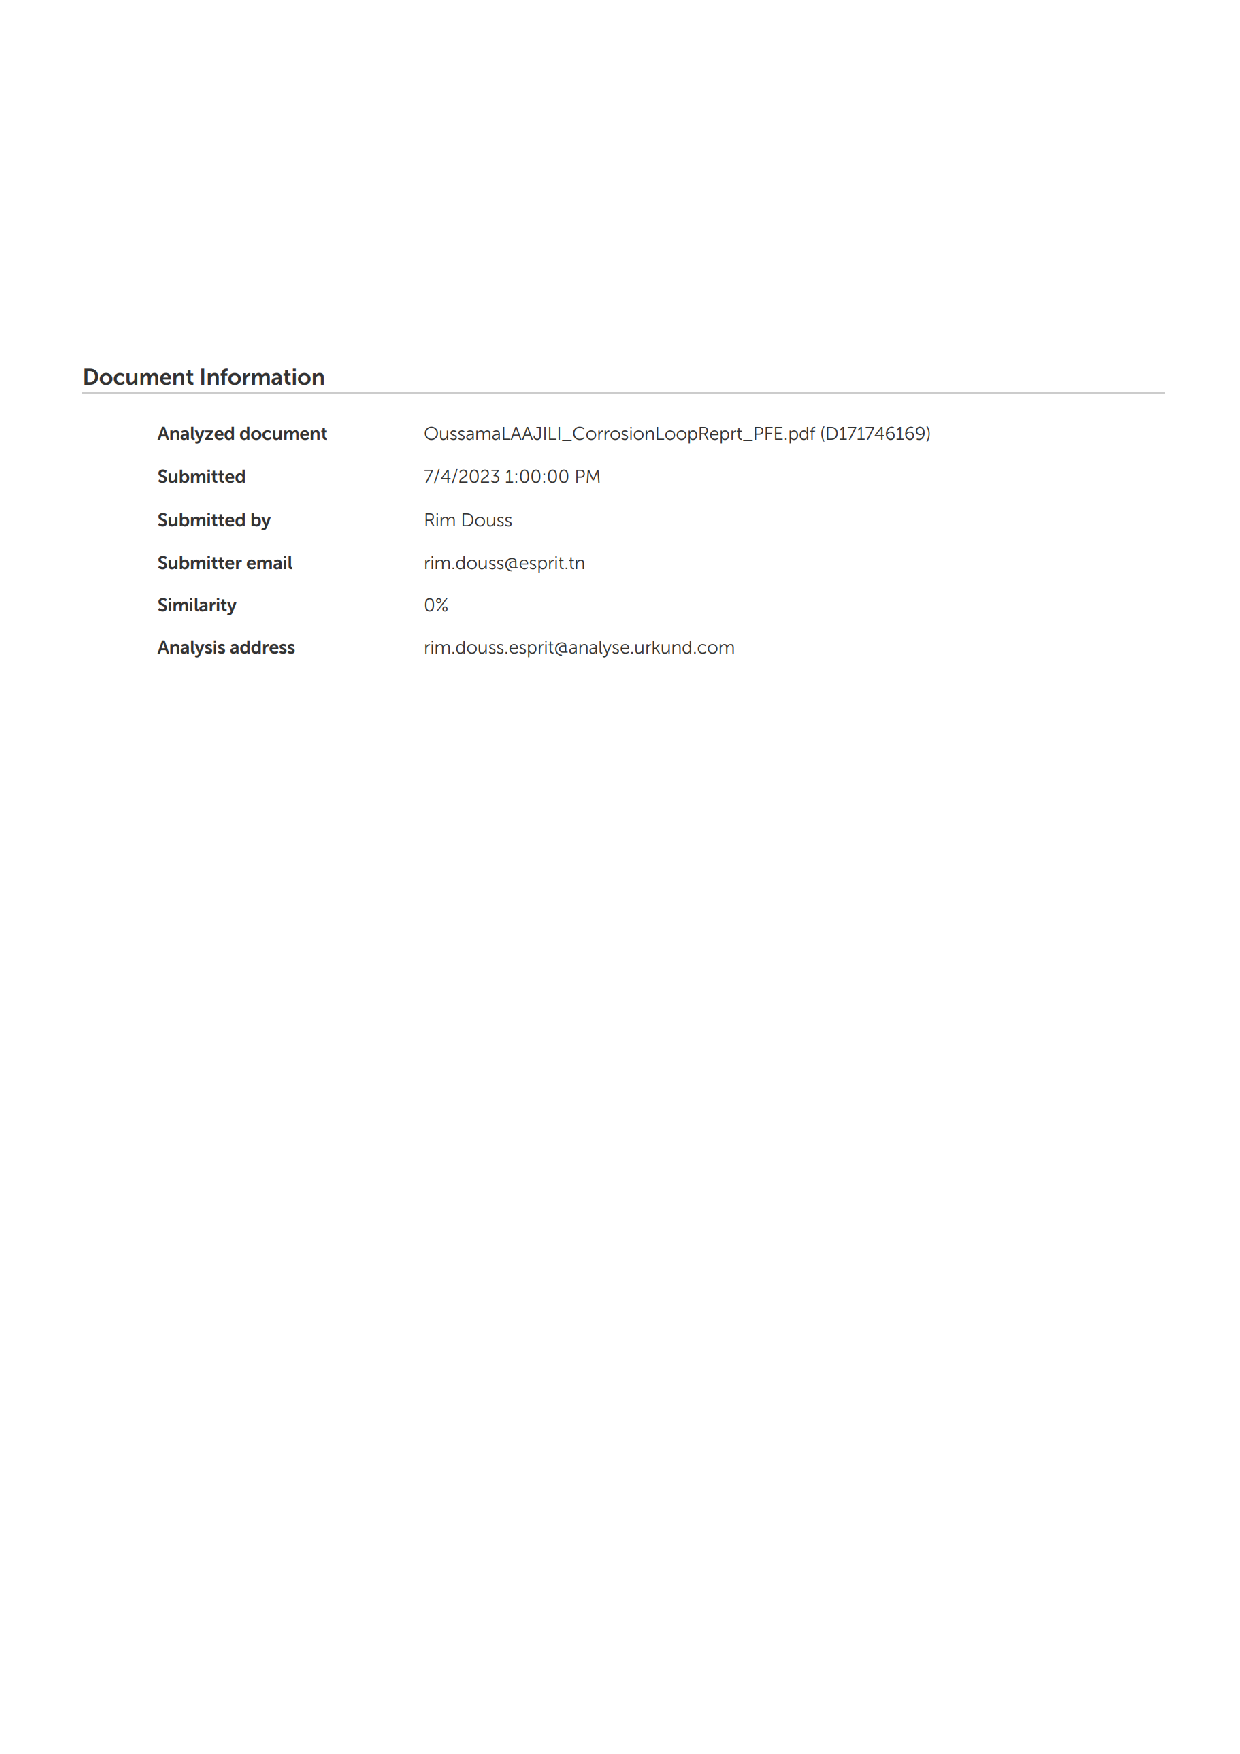
\includepdf[pages=-]{figures/PLAGIAT.pdf}
% \newpage
% \chapter*{\Large \center Dédicaces}

Je dédie ce travail :

\vspace{1em}

\noindent
À mes parents, pour leur amour inconditionnel, leurs sacrifices silencieux et leur soutien constant tout au long de mon parcours académique. Leur confiance m’a donné la force d’aller jusqu’au bout.

\vspace{1em}

\noindent
À ma famille, pour leur présence, leurs encouragements et leur patience, même dans les moments les plus exigeants de ce projet.

\vspace{1em}

\noindent
À mes amis et collègues, pour leur aide, leurs conseils, et les bons moments partagés qui ont rendu cette expérience plus agréable et motivante.

\vspace{2em}


\hfill\textbf {Aziz Aydi}\\

% \chapter*{\Large \center remerciement}

Avant toute chose, je tiens à exprimer ma profonde gratitude à tous ceux qui ont contribué de près ou de loin à la réussite de ce projet de fin d'études.

Je remercie sincèrement \textbf{Madame Houda Jouini Chaabouni}, mon encadrante académique, pour sa disponibilité, ses conseils méthodologiques et son encadrement rigoureux tout au long de cette expérience. Son expertise et ses remarques constructives ont grandement enrichi ce travail.

Je tiens également à remercier \textbf{Monsieur Hichem Aidi}, pour sa confiance, son accompagnement technique et son suivi professionnel qui m'ont permis de m’intégrer dans une logique projet concrète et enrichissante.

Je n’oublie pas l’ensemble du corps professoral de l’école d’ingénieurs \textbf{ESPRIT}, pour la qualité des enseignements dispensés, qui m’ont permis d’acquérir les compétences nécessaires à la réalisation de ce projet.

Enfin, je remercie chaleureusement tous mes collègues, camarades, amis et proches pour leur soutien moral, leur entraide et leurs encouragements constants.

\bigskip

\hfill \textit{À toutes et à tous, merci.}

\hfill\textbf {Aziz Aydi}\\
% \chapter*{\Large \center Introduction générale}

Dans un monde en constante évolution numérique, les plateformes de services à la demande se multiplient pour répondre aux besoins croissants d’efficacité, de flexibilité et de réactivité. Qu’il s’agisse de mise en relation entre particuliers ou de solutions destinées à des structures professionnelles, ces systèmes doivent être pensés pour offrir à la fois une expérience utilisateur fluide, une architecture technique robuste et une évolutivité assurée.

C’est dans ce contexte qu’intervient le projet \textbf{Swift Helpers}, développé dans le cadre de mon projet de fin d’études au sein de la spécialité Génie Logiciel de l’école d’ingénieurs ESPRIT. Ce projet vise à concevoir, développer et déployer une application web complète permettant la gestion d’un réseau de prestataires de services, avec une attention particulière portée à la simplicité d’utilisation, à la modularité technique et à l’automatisation des processus métier.

Le développement de la plateforme s’inscrit dans une démarche agile, structurée en sprints, couvrant toutes les étapes de réalisation : de l’analyse des besoins à l’implémentation des fonctionnalités, jusqu’au déploiement sur un environnement de production Dockerisé. Le système repose sur un backend \textbf{Django REST}, un frontend \textbf{Angular}, une base de données \textbf{PostgreSQL}, et une infrastructure conteneurisée à l’aide de \textbf{Docker}.

Ce projet m’a offert l’opportunité d’appliquer concrètement les compétences acquises tout au long de ma formation, que ce soit en architecture logicielle, en développement fullstack, en conception orientée objet ou en gestion de projet. Il représente également une première immersion dans les exigences réelles d’un système exploitable par des utilisateurs finaux.

Ce rapport présente, dans un premier temps, le contexte général du projet et son périmètre fonctionnel. Il détaille ensuite les différentes phases de développement, organisées par sprint, avant de conclure par le processus de déploiement, les choix techniques effectués, et les perspectives d’évolution du système.





% % -------------------------------------------------------------------
% % Contents, list of figures, list of tables
% % -------------------------------------------------------------------

% \tableofcontents
% \listoffigures





% % -------------------------------------------------------------------
% % Main sections (as required)
% % -------------------------------------------------------------------

% \mainmatter

% \addcontentsline{toc}{chapter}{Abstract} 
% \input{sections/General Context }
% \input{sections/Preliminary Study.tex}
% \input{sections/Specification and Design.tex}
% \input{sections/Realization}
% \input{sections/Results and Discussion.tex}
% \input{sections/Conclusion and Practical Implications.tex}
% \addcontentsline{toc}{chapter}{Conclusion} 
% \input{sections/References.tex}



% % -------------------------------------------------------------------
% % Bibliography
% % -------------------------------------------------------------------



% \printbibliography %Prints bibliography



% % -------------------------------------------------------------------
% % Appendices
% % -------------------------------------------------------------------

% % \begin{appendices}
% % \input{sections/Appendices.tex}
% % \input{sections/appendixB.tex}
% % \end{appendices}

% \newpage
% \thispagestyle{empty}
% \begin{center}
% \end{center}

% \newpage
% \thispagestyle{empty}
% \backgroundsetup{
% scale=1,
% angle=0,
% opacity=1,  %% adjust
% contents={
\includegraphics[width=\paperwidth,height=\paperheight]{figures/back_page.jpg}}
% }
% \begin{center}
% \end{center}
% \end{document}
